\chapter{Le principe d'équivalence}
%Références (qui me fait une bibli mdr) :
%\begin{enumerate}
%    \item Carroll
%    \item Nakahara
%    \item Weinberg
%    \item Misner-Thorne-Wheeler
%    \item Landau-Lifshitz 2
%    \item Notes de cours de Detournay
%    \item Note partielles du cours de FF sur le drive.
%    \item Wikipedia toujours cool 
%    \item Je recommande la série \emph{Tensors Calculus} de la chaine YouTube \emph{eigenchris}.
%    \item MIT 8.962 General Relativity (enregistrements YouTube)
%    \item Blau (vrmt cool mais long)
%    \item Hawking-Ellis
%\end{enumerate}

\section{Origine de la relativité générale}


\subsection{Nécéssité d'une théorie de relativité générale}
Parfois, l'élaboration de théories physiques est guidée par l'expérience. Un champ électrique $\vect{E}$ va générer une tension dans un fil et y faire circuler un courant. D'autre part, on observe qu'un champ magnétique $\vect{B}$ variable engendre un courant induit. Les champs $\vect{E}$ et $\vect{B}$ doivent donc être reliés par les équations décrivant ces phénomènes : les équations de Maxwell (environ 1861).
Dans d'autres cas, de nouvelles théories émergent à cause d'\emph{incompatibilités} ou de \emph{contradictions} entre des théories existantes. Dans ce dernier cas, deux théories peuvent être parfaitement valides dans leurs domaines respectifs, mais conduire à des contradictions lorsqu'elles sont combinées. La relativité générale appartient à ce deuxième cas. Donnons quelques exemple de ce cas de figure :

\begin{enumerate}
    \item \textbf{La catrastophe UV et la mécanique quantique}\\ 
    la thermodynamique classique (via le théorème d'équipartition), combinée aux lois de l'électromagnétisme (Maxwell), prédit une divergence de l'énergie d'un corps noir : la catrastophe UV. En 1900, Max Planck résout ce paradoxe en postulant que l'énergie électromagnétique est émise par quanta $E = n h \nu$, marquant ainsi le premier pas vers la \emph{mécanique quantique}.\\
    \item \textbf{Le paradoxe du miroir d'Einstein et la relativité restreinte}\\
    La \emph{relativité restreinte} d'Einstein (1905) est quant à elle née des contradictions qui existaient entre les équations de Maxwell (vitesse de la lumière absolue $c$) et les lois du mouvement de Galilée (tous les mouvements sont relatifs, addition des vitesses). Einstein imagina l'expérience de pensée suivante : s'il courait à la vitesse de la lumière avec un miroir dans les mains devant lui, verrait-il la réflexion de son visage ? Selon les équations de Maxwell, on ne verrait rien, car la lumière de son visage n'arrivera pas à atteindre le miroir. Selon la relativité Galiléenne par contre, on ne peut distinguer entre référentiels inertiels : on se verrait aussi bien qu'au repos. Einstein résoud ce paradoxe en introduisant la relativité restreinte en 1905.\\
    \item \textbf{La théorie quantique des champs}\\
    En mécanique quantique non-relativiste, un système est décrit par des degrés de liberté fixes. Néanmoins, la relation $E=mc^2$ implique que la création de particules est possible à énergie suffisemment grande, donnant lieu à une variation des degrés de liberté du système. Cela exige un formalisme plus général : la théorie quantique des champs.
\end{enumerate}
\begin{center}
    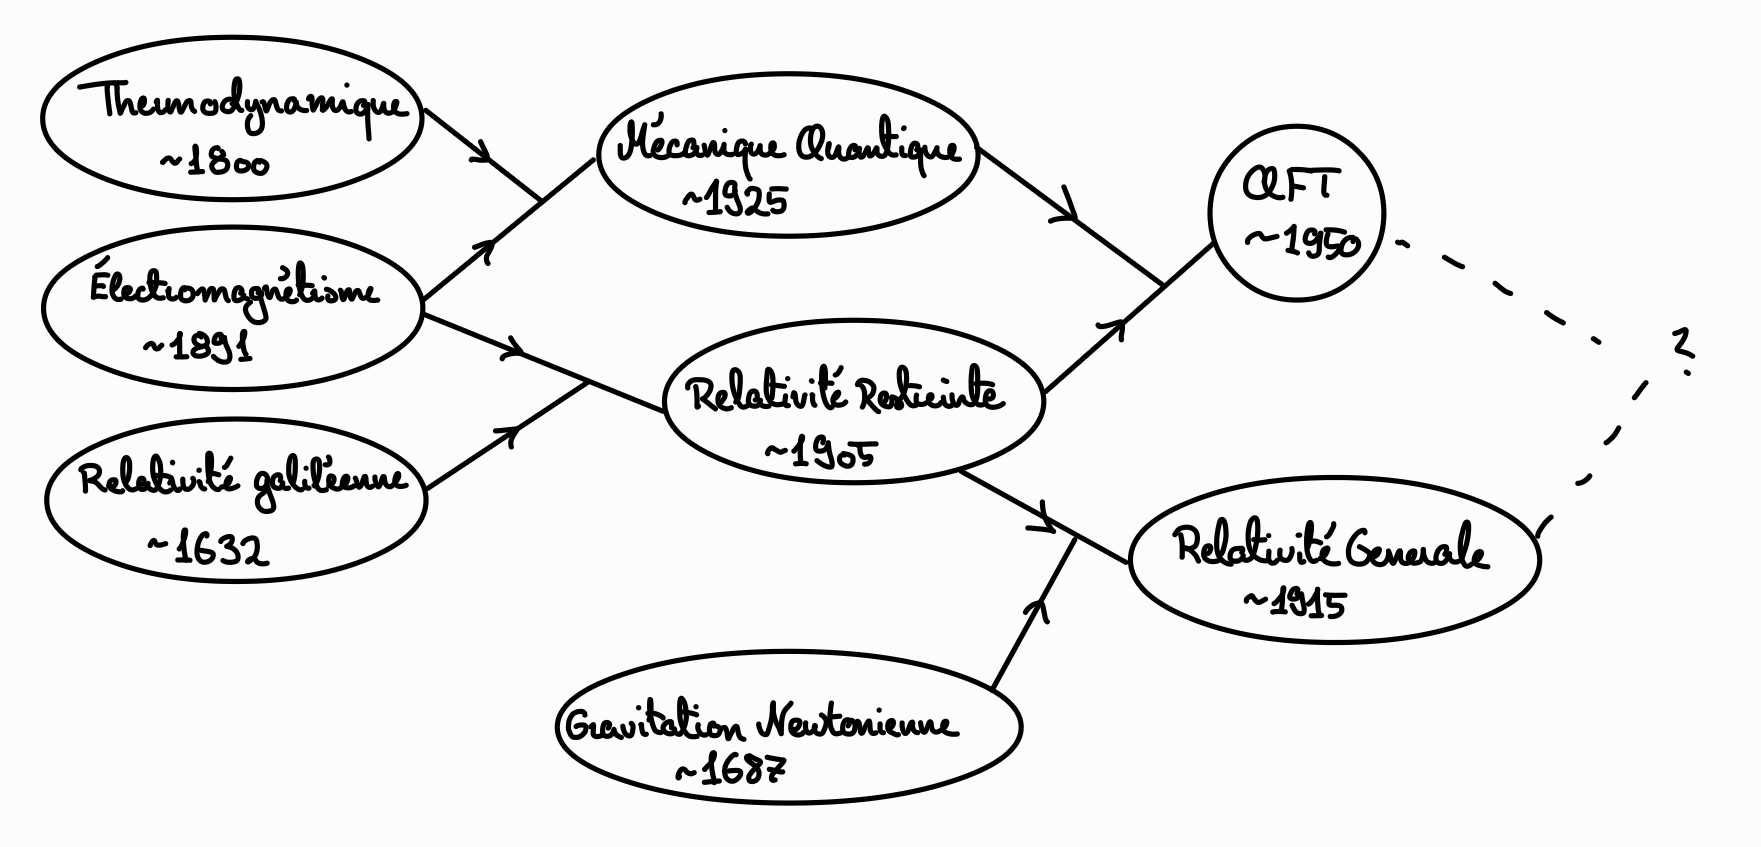
\includegraphics[scale=0.2]{Chapitres/1. Introduction/Images/Contradictions temp.png}
\end{center}
\begin{center}
    \textit{Contradictions equal progress.} (temp graph)
\end{center}
Il est intéressant de noter que la plupart des découvertes rappelées ci-dessus émergent plus d'\emph{expériences de pensée} plutôt que de réelles exprériences de laboratoire qui ont abouti à des révolutions. Einstein sera souvent guidées par celles-ci, comme il le fût pour la relativité restreinte, pour établir les principes de la relativité générale.
\begin{center}
    \textit{Je tiens pour vrai que la pensée pure est compétente pour comprendre le réel.}
    
    \noindent \emph{Ma conviction est que nous sommes en mesure, grâce à une construction purement mathématique, de trouver les concepts, ainsi que les lois qui les relient, propres à nous ouvrir les portes de la compréhension des phénomènes natures.}
\end{center}
\begin{flushright}
    - Albert Einstein
\end{flushright}
\subsection{L'incompatibilité de la relativité restreinte et la gravitation newtonienne}
Dans le cas de la relativité générale (RG), les théories qui ont poussées à sa création sont la relativité restreinte (RR) et la loi de gravitation universelle de Newton. Pour rappel, cette dernière stipule qu'un corps de masse $m$ soumis uniquement à l'attraction gravitationnelle d'un corps de masse $M$ subit une force
\begin{equation}
    \vect{F} = -G \, \frac{M m}{r^2}\,\vect{u}\indices{_r} \deq m\,\vect{g}\indices{_M}
\end{equation}
où $G$ est la constante de gravitation universelle, $r$ est la distance qui sépare les deux masses et $\vect{g}\indices{_M}$ le champ gravitationnel produit par la masse $M$.\\
Bien que cette théorie ait connu un immense succès pendant plus de deux siècles, elle présente plusieurs incompatibilités avec la relativité restreinte. En voici quelques-unes :

\begin{enumerate}
    \item \textbf{Propagation instantanée de la gravitation} \\
    Imaginons que le soleil disparaît à un moment donné. Selon la loi de gravitation newtonienne, la force gravitationelle s'annulera instantanément (comme $M=0$). Or, la relativité restreinte indique que aucune information ne peut se propager plus vite que la lumière, qui prend 8 minutes pour parvenir à la Terre. La vitesse de propagation de la force gravitationnelle serait donc $v = \infty > c$.\\
    
    \item \textbf{Non-invariance de Lorentz}\\
    La force de gravitation $\vect{F}$ est invariante sous transformations de Galilée 
    \begin{align}
        \begin{dcases}
            t' = t \\
            x' = x - vt\\
            y' = y\\
            z'=z
        \end{dcases}
    \end{align}
    car la quantité $r^2 = (\vect{x}_m - \vect{x}_M )^2 $ est conservée. Néanmoins, elle n'est pas invariante sous les transformations de Lorentz reliant deux observateurs inertiels :
    \begin{align}
        \begin{dcases}
            t' = \gamma(t - \frac{v}{c^2}x) \\
            x' = \gamma(x - vt)\\
            y' = y\\
            z'=z
        \end{dcases}
    \end{align}

    avec le facteur de Lorentz $\gamma = \dfrac{1}{\sqrt{1 - \frac{v^2}{c^2}}}$. \\
    
    \item \textbf{Non-linéarité d'une théorie relativiste de la gravitation}\\
    D'après la relativité restreinte, la masse est seulement une autre forme d'énergie. Ainsi, puisque la gravité couple à la masse (la masse est la \emph{charge gravitationnelle}), elle doit aussi coupler à l'énergie dans une théorie relativiste. Autrement dit, le contenu en énergie du système affecte le champ de gravitation. En particulier, la gravité devra coupler à l'énergie gravitationnelle, donc à elle-même. Les nouvelles équations du champ gravitationnel (\ref{eq:Einstein introduction}) seront intrinsèquement non-linéaires : le champ dû à la somme de deux masses n'égale pas la somme des champs gravitationnels des deux masses isolées, car l'énergie gravitationnelle d'interaction du système doit être pris en considération.\\
    
    Comparativement, l'équation de Poisson pour un potentiel gravitationnel newtonien s'écrit : 
    \begin{equation}
        \Delta \Phi = 4\pi G \,\rho
    \end{equation}
    où $\Phi$ est le potentiel gravitationnel (énergie) et $\rho$ est la masse volumique. En relativité restreinte, la densité $\rho$ devient alors dépendante de $\Phi$. On dit alors que la gravité est \emph{bouclée sur elle-même}. \\
 \end{enumerate}
 De plus, on peut se poser une question \emph{d'équivalence des référentiels} : en relativité galiléenne, il semble que les référentiels intertiels jouent un rôle privilégié : les lois de la physique y sont plus simples. Pourquoi une telle classe de référentiels existerait-elle ? De plus, il y a l'ambiguité du choix d'un premier référentiel intertiel, comme nous ne pouvons pas définir celui-ci de manière absolue. \\
 La relativité générale répond à ces questions en affirmant que \emph{tous} les référentiels sont équivalents pour la formulation des lois physiques, qu'ils soient inertiels ou non.

Avec ces ces inconsistence en tête, Einstein se lança dans la tâche d'incorporer l'interaction gravitationnelle en une théorie relativiste. Max Planck, ayant eu vent de l'entreprise d'Einstein lui aurait écrit :
\begin{center}
    \textit{As an older friend, I must advise you against it for, in the first place you will not succeed, and even if you succeed, no one will believe you.}
\end{center}
Et d'autre part :
\begin{center}
    \textit{When a serious scientist tells you something can be done, he's must likely to be right; But when he tells you it cannot be done, he's most likely to be wrong.}
\end{center}
Et il se fait qu'Einstein était têtu.
\subsection{Comparaison avec l'électromagnétisme}
La loi de gravitation newtonienne possède une forme remarquablement proche de la loi de Coulomb (électrostatique) :
\begin{align}
    \vect{F} = \frac{1}{4\pi \varepsilon_0} \frac{Q q}{r^2} \,\vect{u}\indices{_r} = q \,\vect{E}_q
\end{align}
Cette similarité soulève une question importante : pourquoi l'électromagnétisme ne souffre-t-il pas des mêmes problèmes que ceux évoqués pour la gravitation newtonienne ? La réponse réside simplement dans le fait que  la loi de Coulomb n'est qu'un cas particulier des équations de Maxwell qui, quant à elles, sont bien compatible avec la relativité restreinte. 
\begin{rap}
    Le quadri-potentiel électromagnétique $A^\mu = (\phi/c,\vect{A})$ s'écrit en fonction des champs $(\vect{E},\vect{B})$ selon :
    \begin{align}
        \begin{dcases}
            \vect{E} = - \vect{\nabla} \phi - \frac{\pd \vect{A}}{\pd t} \\
            \vect{B} = \vect{\nabla} \times \vect{A}
        \end{dcases}
    \end{align}
    Le champ électromagnétique peut donc être complètement décrit par les potentiels $(\vect{A},\phi)$. 
\end{rap}
\begin{rap}
    Le \emph{tenseur de Faraday} (également appelé le \emph{tenseur d'intensité du champ EM}) est un tenseur complètement anti-symmétrique donné par
    \begin{equation}
    \label{eq:Farady intro}
        F\indices{_\mu_\nu} \deq \pd_\mu A_\nu - \pd_\nu A_\mu
    \end{equation}
\end{rap}
\begin{exerc}
    Trouvez à partir de \ref{eq:Farady intro} la relation du tenseur de Faraday et les champs $(\vect{E},\vect{B})$.
\end{exerc}
\cutebreak
Armé de ces définitions, les équations de Maxwell peuvent être exprimées sous une forme tensorielle\footnote{Nous reviendrons sur cette formulation plus en détail dans la suite du cours. En particulier, la notation $[]$ sur les indices peut être ignorée pour le moment.} :
\begin{align}
    \begin{dcases}
        \pd\indices{_\mu} F\indices{^\mu^\nu} = J\indices{^\nu} \\
        \partial\indices{_[ _\alpha} F\indices{_\mu_\nu _]} = 0
    \end{dcases}
\end{align}
où $J^\mu = (c \rho,\vect{A})$ est le quadri-courant. Dans cette forme, les équations de Maxwell sont manifestement invariantes de Lorentz\footnote{Pour être tout à fait exact, il s'agit d'une covariance. De nouveau, nous y reviendrons plus tard.}.
\\
Vu qu'il s'agit d'équations tensorielles (pour des transformations de Lorentz), elles sont valables dans n'importe quel référentiel inertiel, et leur covariance est immédiate (voir ci-dessous).
\begin{itemize}
    \item \textbf{Loi de transformation de la force de Coulomb}\\
    À partir des équations de Maxwell, il est facile de montrer la force agissant sur une particule de charge $q$ se déplaçant à vitesse $\vect{v}$ dans des champs $(\vect{E},\vect{B})$ est donnée par la force de Lorentz :
    \begin{equation}
        \vect{F} = q\,  (\vect{E} + \vect{v} \times \vect{B})
    \end{equation}
    Nous verrons qu'en notation tensorielle, cette force s'écrit 
    \begin{equation}
        F^\alpha = q \, u_\beta F\indices{^\alpha ^\beta}
    \end{equation}
    où $u_\beta$ est la quadri-vitesse de la particule, et la force étant donné en fonction de la quadri-impulsion $P^\alpha = (\gamma m c, m \vect{v})$ selon :
    \begin{equation}
        F^\alpha \deq \frac{\td P\indices{^\alpha}}{\td \tau}
    \end{equation}
    où $\tau$ est le temps propre de la particule. La force de Coulomb étant un quadri-vecteur (et pas un scalaire), elle n'est \emph{pas} invariante sous transformation de Lorentz. Par contre, elle est \emph{covariante} : la connaissant dans un réfénrentiel de Lorentz (inertiel), on peut la connaître dans tout référentiel de Lorentz car elle obéit à une loi de transformation précise (ici $F^\alpha \to \Lambda\indices{^\alpha_\!_\beta}F^\beta$).\\
    \item \textbf{Quid de la propagation instantanée ?}\footnote{Wald p.78}\\
    Un changement drastique se produit lorsqu'on passe de la théorie électrostatique de Coulomb aux équations de Maxwell : le champ électromagnétique $A_\mu = (\phi/c, - \vect{A})$ (avec $\vect{E} = - \vect{\nabla} \phi - \frac{\pd \vect{A}}{\pd t}$ et $\vect{B} = \vect{\nabla} \times \vect{A}$) devient une entité dynamique. En particulier, les équations de Maxwell dans le vide admettent des solutions ondulatoires, et la radiation électromagnétique peut se propager librement à la vitesse
    \begin{equation}
        v = c = \frac{1}{\sqrt{\varepsilon_0\mu_0}}
    \end{equation}
    dans le vide.
\end{itemize}
\begin{rmk}
    La théorie quantique des champs (QFT) nous indique de décrire les processus élémentaires en termes de particules élémentaires et de leurs collisions. En électrodynamique classique, ce sont les solutions ondulatoires des équations de Maxwell qui mènent le plus naturellement à une interprétation en termes de particules : le photon ($A_\mu$) se propageant à vitesse $c$. L'interaction n'est plus instantanée, et se fait via des perturbations du champ EM $A_\mu$ (qui se propagent à vitesse $c$), ou via échange de photons dans la théorie quantique.
\end{rmk}
\begin{rmk}
    Un changement similaire se propduira pour la gravitation en passant de Newton à la relativité générale. Cette dernière admet des solutions ondulatoires dans le vide (les \emph{ondes gravitationnelles}) se propageant à vitesse $c$ et sont également associées à une particules : le \emph{graviton}.
\end{rmk}
La loi de Coulomb a donc l'avantage de dériver d'un cadre plus fondamental, dans lequel les problèmes liées à la propagation et à l'invariance sont résolues. En gravitation, notre objectif sera de construire une théorie similaire, cohérente avec la relativité restreinte. Dans cette théorie, la gravitation newtonienne ne sera qu'une approximation valable dans un régime particulier.

\section{Principe d'équivalence}
La théorie de gravitation d'Einstein repose en grande partie sur une idée conceptuellement simple, appelée le \emph{principe d'équivalence} (PE). Einstein lui-même la qualifia de \emph{l'idée la plus heureuse de sa vie}. Nous rencontrerons ce principe à plusieurs reprises. Dans cette introduction, nous en donnerons une version littéraire, avant d'attaquer des formulations plus mathématiques dans les chapitres suivants. Certaines références différencient plusieurs formulations du PE. Voici-en un bref apperçu :
\begin{itemize}
    \item \textbf{Le PE faible} \\
    Postule l'équivalence entre masse inertielle et masse gravitationnelle (discuté dans la section \ref{sec:PE1} qui suit).\\
    \item \textbf{Le PE d'Einstein}\\
     Forme principale du principe d'équivalence dans la relativité générale, que nous adopterons dans ce cours (voir section \ref{sec:PE2}).\\
    \item \textbf{Le PE fort} \\
    Modification subtile du PE d'Einstein, impliquant un couplage de la gravitation avec elle-même. Cette formulation ne sera pas discutée dans ce cours.
\end{itemize}
Dans la suite du cours, nous désignerons par \emph{principe d'équivalence} uniquement la formulation d'Einstein.
\subsection{Préliminaires}
\label{sec:PE1}
Avant d'attaquer la formulation explicite du PE, formulons les observation fondamentales suivantes, distinguant l'interaction gravitationnelle d'autres types d'interactions.

Avant d'introduire formellement le principe d'équivalence (PE), posons quelques observations fondamentales, vérifiées expérimentalement, qui distinguent l'interaction gravitationnelle des autres types d'interactions.
\begin{theoremframe}
    \begin{propri}
        \label{post:PE1}
        L'effet de la gravité est \textbf{universel}. Tous les corps sont affectés de la même manière par la gravité, indépendamment de leur masse, charge, composition, etc.
    \end{propri}
\end{theoremframe}
Cette universalité fut mise en évidence pour la première fois par Galilée, dans sa fameuse expérience de la chute des corps. Cette expérience est illustrée plus récemment par la mission \textsc{Apollo 15} en 1971.
\begin{theoremframe}
    \begin{propri}
        \label{post:PE2}
        La gravité est toujours attractive.
    \end{propri}
\end{theoremframe}
En particulier, la gravité ne peut pas être écrantée. Cela la distingue fondamentalement de l'électromagnétisme, où il existe des charges positives et négatives. Cet écrantage est illustrée en EM par la cage de Faraday.

\begin{rmk}
    La propriété \ref{post:PE1} implique\footnote{Ou plus précisément, une justification de cette propriété est} l'égalité entre la masse inertielle $m_i$ et la masse gravitationnelle $m_g$. La première apparaît dans la deuxième loi de Newton $\vect{F} =m_{i}\vect{a}$, alors que la seconde est définie par la loi de gravitation newtonienne $\vect{F} =m_{g}\vect{g}_\mathbf{M}$. En supposant que le corps est soumis uniquement à un champ gravitationnel, nous avons :
    \begin{equation}
        \vect{a} = \frac{m_g}{m_i} \, \vect{g}
    \end{equation}

    Expérimentalement, nous n'observons aucune différence entre ces deux paramètres, alors qu'a priori, ils n'ont aucun lien. D'après les dernières mesures (le satellite \textsc{Microscope}) :
    \begin{equation}
        \left| 1 - \frac{m_i}{m_g} \right| \lesssim 10^{-14}
    \end{equation}
    Tous les corps chutent avec la même accélération dans un champ gravitationnel, indépendamment de leur \emph{charge gravitationnelle} : $\vect{a} = \vect{g}$. En comparaison, l'interaction électromagnétique montre un comportement très différent :
    \begin{equation}
        \vect{F} = q \, \vect{ E} \iff \vect{a} = \frac{q}{m_i} \, \vect{E}
    \end{equation}
    qui dépend explicitement de $q$ et $m_i$.
\end{rmk}
\begin{rmk}
    Le postulat \ref{post:PE2} permet d'expliquer pourquoi l'interaction gravitationnelle est observable à des échelles macroscopiques malgré son extrême faiblesse :
    \begin{equation}
        \left| \frac{F_g}{F_e}\right| \sim 10^{-43}
        \label{force gravité}
    \end{equation}
    Contrairement, l'interaction EM n'a pas d'effets macroscopiquement importants, car ceux-ci s'estompent par écrantage (corps macroscopiquement neutres).
\end{rmk}
\begin{center}
        \textit{La gravité est partout et affecte tous les corps de la même façon.}
    \end{center}
\subsection{L'ascenseur d'Einstein}
Einstein eut l'intuition que l'équivalence entre masse inertielle et masse gravitationnelle, loin d'être une coïncidence, indiquait quelque chose de fondamental sur la nature de la gravitation : la gravité et l'inertie (ou l'accélération) seraient \emph{indistinguables}. Il illustra cette idée par la célèbre expérience de pensée suivante.

\subsubsection{Gravité et inertie}
Supposons qu'une personne se trouve dans une boite isolée de l'extérieur (disons, un ascenseur). Lorsqu'elle lâche un objet, celui-ci tombe vers le sol (disons, accéléré uniformément). Deux conclusions lui sont possible à partir de cette interprétation :
\begin{itemize}
    \item L'objet retombe sous l'effet d'un champ gravitationnel, alors que l'ascenseur est immobile.
    \item L'objet retombe par effet d'inertie : l'ascenseur accélère vers le haut alors que l'objet relâché reste immobile du point de vue d'un observateur extérieur. 
\end{itemize}
\begin{center}
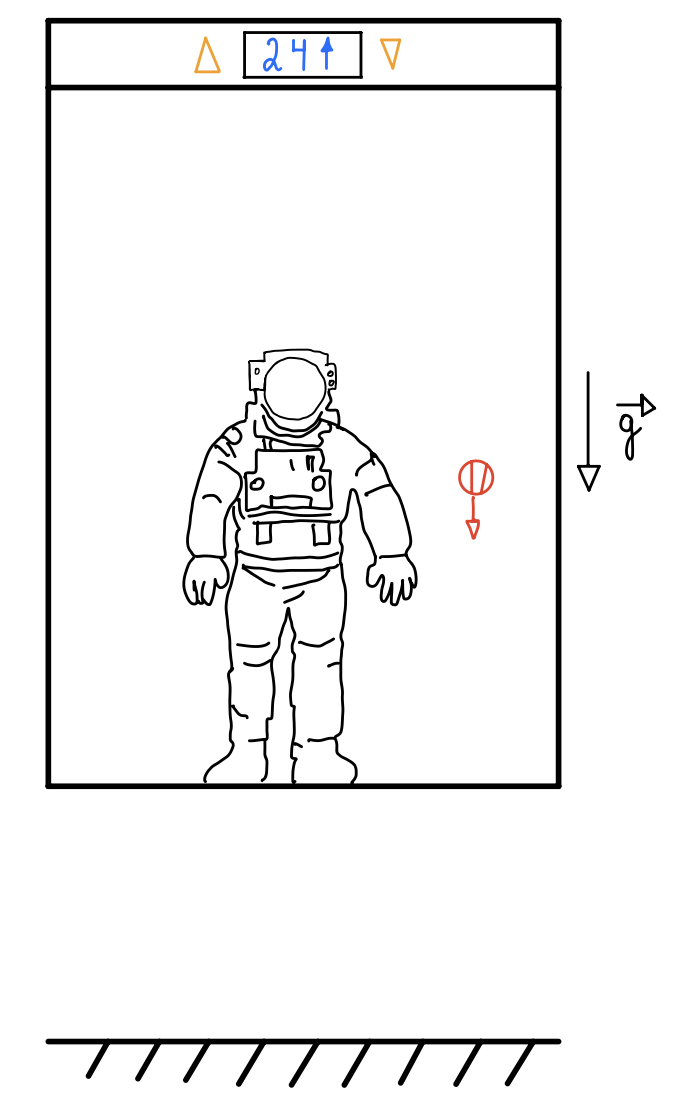
\includegraphics[scale=0.2]{Chapitres/1. Introduction/Images/homme ascenseur.png}
\includegraphics[scale=0.2]{Chapitres/1. Introduction/Images/homme fusée.png}
\end{center}
Du point de vue de l'observateur à l'intérieur, confiné à une petite région de l'espace, la gravité et l'accélération uniforme sont indistinguables, qui est confinée dans une petite région. 

\subsubsection{Apesanteur et chute libre}
Supposons à présent que lorsque la personne lâche l'objet, celui-ci reste immobile (ne tombe pas) du point de vue de la personne. À nouveau, deux conclusions lui sont possibles :
\begin{itemize}
    \item L'ascenseur est situé dans l'espace, loin du champ de gravitation : il est en apesanteur. L’objet flotte simplement car il n'est soumis à aucune force. On dit qu'il suit une \emph{trajectoire libre}.
    \item L'ascenseur est en chute libre dans le champ de gravitation terrestre. Le poids effectif de la personne et de l'objet est nul ($\vect{P} = m(\vect{g} + \vect{a})$ mais en chute libre, $\vect{a} = - \vect{g}$ et donc $\vect{P} = 0$).
\end{itemize}
Dans les deux cas, l'objet flotte dans l'ascenseur. Les effets de la gravité peuvent donc être annulés \emph{localement} (à l'intérieur de l'ascenseur) en se plaçant dans un référentiel en chute libre, i.e. le référentiel de l'objet qui est soumis à cette force gravitationnelle.

\begin{center}
\includegraphics[scale=0.2]{Chapitres/1. Introduction/Images/homme fussée apesenteur.png}
\end{center}
\begin{rmk}
    Notons que jusqu'à présent, toutes ces observations restent valable dans la théorie Newtonienne. En effet, il est possible d'annuler localement la force de gravitation. Il suffit seulement de changer de référentiel pour se mettre dans un référentiel avec une accélération égale à la force de gravitation : étant donné $\ddot{x} = g$ :
    \begin{align}
        \xi(t,x) = x - g \frac{t^2}{2}
    \end{align}
    Qui est tel que $\ddot{\xi} = 0$.
\end{rmk}
\cutebreak
Dans ce référentiel \emph{en chute libre}, et puisque les effets de la gravité ont été annulés pour tout ce que contient l'ascenseur, ce sont les lois physiques habituelles en l'absence de gravité qui sont appliquables. Inversément, en connaissant les lois physiques en l'absence de gravité, on devrait pouvoir les déterminer en présence de gravité grâce à la transformation permettant de passer d'un référentiel en chute libre à un référentiel général.
\subsection{Les deux formulations du principe d'équivalence}
\label{sec:PE2}
\begin{theoremframe}
    \begin{propri}[Principe d'équivalence, première version]
        En tout point de l'espace-temps, il est possible de choisir un système de coordonnées tel que localement autour de ce point, les lois de la physique prennent la même forme qu'en l'absence de gravitation dans un référentiel inertiel.
    \end{propri}
\end{theoremframe}
Un tel référentiel, dit \emph{en chute libre}, est appelé un référentiel localement inertiel (RLI).
\begin{theoremframe}
    \begin{propri}[Principe d'équivalence, deuxième version]
        Localement, aucune expérience ne permet de distinguer un champ de gravitation et une accélération uniforme. 
    \end{propri}
\end{theoremframe}
Notons que la notion \emph{locale} utilisé ici peut se définir d'une manière mathématiquement précise, sur laquelle nous reviendrons plus tard. Pour le moment, il est seulement important de retenir que l'équivalence entre gravitation et accélération n'est valable que dans des régions suffisamment restreintes de l'espace-temps, sans quoi les inhomogénéités du champ gravitationnel feront que l'effet sur des \emph{particules-test} ou objets environnants sera différent d'un référentiel accéléré uniformément.

% Image cf notes
Cet impossibilité de distinguer localement les effets d'un champ de gravitation d'une accélération uniforme est un phénomène de la relativité générale analogue à l'impossibilité en relativité galiléenne de mesurer la vitesse absolue d'un observateur.

\subsection{Conséquence : le redshift gravitationnel}
Une célèbre prédiction du PE est le \emph{redshift gravitationnel}, c’est-à-dire une modification de la fréquence d’un signal lumineux lorsqu’il traverse un champ gravitationnel.
\subsubsection{2.4.1 Accélération uniforme et effet Doppler}
Considérons deux fusées séparées d'une distance $z$ et ayant une accélération relative uniforme $\vect{a}$. À l'instant $t_0=0$, un photon est émis par la fusée 1, qui, à cet instant, se déplace à une vitesse $v$. On souhaite calculer le redshift (par effet Doppler) qu'aura le signal quand il arrivera à la fusée 2 au temps $t_0 + t^*$. Comme l'accélération est constante, on a :
\begin{align}
    z(t) = z_0 + vt + \frac{at^2}{2}
\end{align}
En supposant que $v \ll c$, un rapide calcul montre que $t^* = z(t^*)/c$ (exercice d'échauffement). En $t_0+t^*$, la vitesse de la fusée réceptrice est 
\begin{equation}
    v+at^*=v+\frac{az}{c}.
\end{equation}

\begin{center}
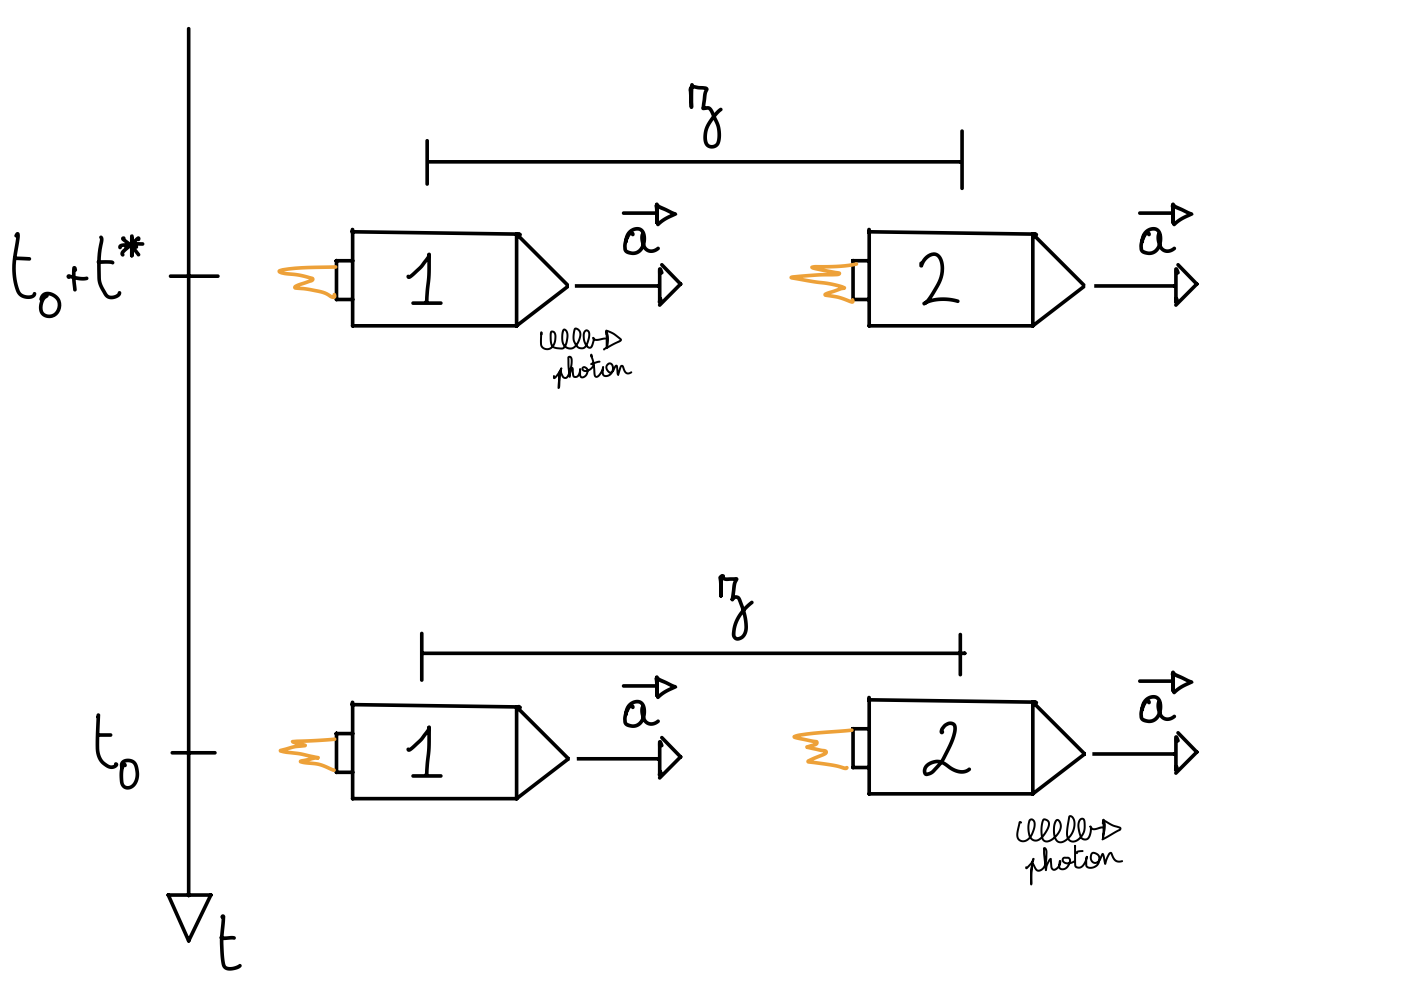
\includegraphics[scale=0.3]{Chapitres/1. Introduction/Images/photon.png}
\end{center}
L'émetteur et le récepteur n'ayant pas la même vitesse, la fréquence perçue par le récepteur va être modifié par effet Doppler :
\begin{align}
    \frac{\Delta\lambda}{\lambda_1}& = \frac{\lambda_2 - \lambda_1}{\lambda_1} = \frac{\Delta v}{c} = \frac{az}{c^2} \\
    &= \frac{\Delta T}{T_1} =\frac{\Delta \tau_2 - \Delta \tau_1}{\Delta \tau_1}
\end{align}
Comme $\delta v > 0$ on aura $\Delta \tau_2 > \Delta \tau_1$. En imaginant que le signal envoyé correspond à l'horloge interne de la fusée 1, on conclut que \emph{le temps s'écoule plus vite pour la fusée 2} . 

\subsubsection{2.4.2 Champ gravitationnel et effet Doppler}
En vertu du PE, la même phénomène doit se produire dans un champ de gravitation uniforme $g$. Supposons qu'une personne se trouve en haut d'une tour à hauteur $z_2$ et une deuxième personne en bas de la tour à une hauteur $z_1$ envoie un signal $\lambda_1$ vers la personne en haut de la tour. 

\begin{center}
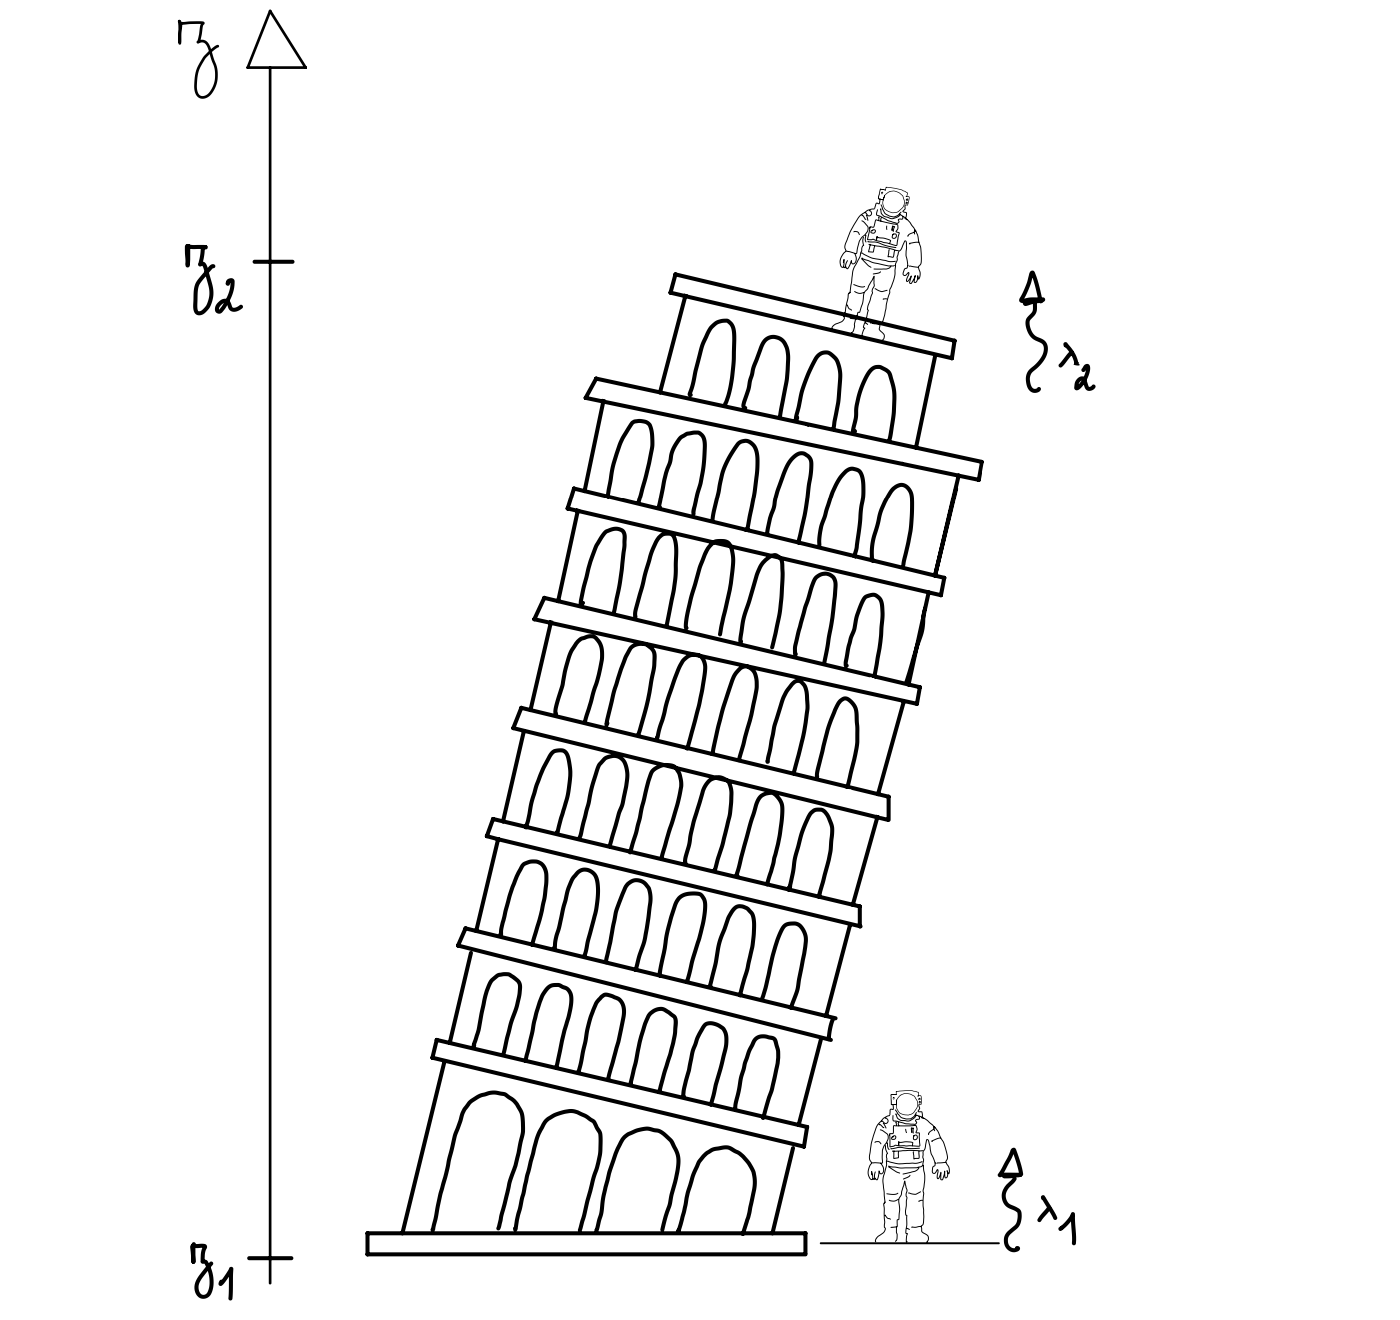
\includegraphics[scale=0.3]{Chapitres/1. Introduction/Images/Tour.png}
\end{center}
Comme les deux situations sont indistinguables, on doit trouver :
\begin{equation}
    \frac{\Delta \lambda}{\lambda} = \frac{\Delta T}{T} = \frac{g(z_2 - z_1)}{c^2}>0
\end{equation}
Et on trouvera donc que $T_2 > T_1$, c'est-à-dire que la période mesuré en haut de la tour sera plus grande que celle mesuré en bas de la tour. 

En conclusion, dans un champ de gravitation, la période du signal n'est pas la même au pied de la tour que en haut de la tour. Le temps s'écoule plus lentement le plus le champ de gravitation est fort\footnote{cf. \emph{Interstellar} lorsqu'iels se rapprochent du trou noir.}. Il s'agit d'un \textit{redshift gravitationnel}. 

\subsection{Remarque sur la nature géométrique de l'espace-temps en présence de gravitation}
Le redshift gravitationnel a une interprétation importante quant à la nature même de l'espace-temps. Supposons à présent qu'on envoie une onde périodique vers le haut de la tour, dont deux fronts d'onde sont séparés d'un temps $\Delta t_1 = \lambda_1/c$. Par contre, en haut de la tour, le signal reçu possède une période $\Delta t_2 = \lambda_2/c > \Delta t_1$, en vertu du redshift gravitationnel. Mais si le champ de gravitation est statique, c'est-à-dire indépendant du temps (ce qu'on a supposé implicitement jusqu'à ici), les chemins suivis dans l'espace-temps par les trains d'onde successifs A et B doivent être congruents (parallèles) quelle que soit la forme précise de ces chemins (que l'on ne prétend pas connaître en présence de gravitation). Alors, on devrait nécessairement avoir $\Delta t_1 = \Delta t_2$, mais ce n'est pas le cas ! \\
\\
Une interprétation est que l'espace-temps à travers lequel les photons se propagent est courbe. En effet, dans un espace plat (par exemple l'espace Euclidien $\R^3$), deux trajectoires initialement parallèles conservent leur séparation au cours du temps. En revanche, en présence de courbure, cette propriété n'est plus garantie. Par exemple, sur la sphère $S^2$, deux \emph{lignes} (géodésiques) initialement parallèles ne conservent pas la distance entre-eux, et finiront même par se croiser !

On ne peut pas à strictement parler \emph{prouver} que l'espace-temps est courbe (pas plus qu'on ne peut \emph{prouver} les lois de Newton). On peut par contre envisager l'hypothèse, d'en déduire des prédictions qui l'infirmeront ou la confirmeront. Nous allons donc être amenés à développer des outils permettant de décrire des espaces-temps courbes, mais qui localement \emph{ressemblent} à l'espace-temps plat de (Poincaré) Minkowski, puisque localement dans un référentiel approprié, la relativité restreinte doit y être applicable.

Imaginons à présent que le premier signal à période $T_0$ arrive en haut de la tour avec une période $T_0+T_1$. Que se passerait-il si un deuxième signal est renvoyé du bas de la tour avec une fréquence de $T_0+T_1$ ? En supposant une gravitation statique, il serait évident de conclure que la différence en fréquence $T_2 = T_1$. Néanmoins, cet argument n'est applicable que si l'espace-temps est plat. Nous verrons dans la suite que si $T_2 \neq T_1$, alors l'espace-temps est courbe.

\begin{center}
    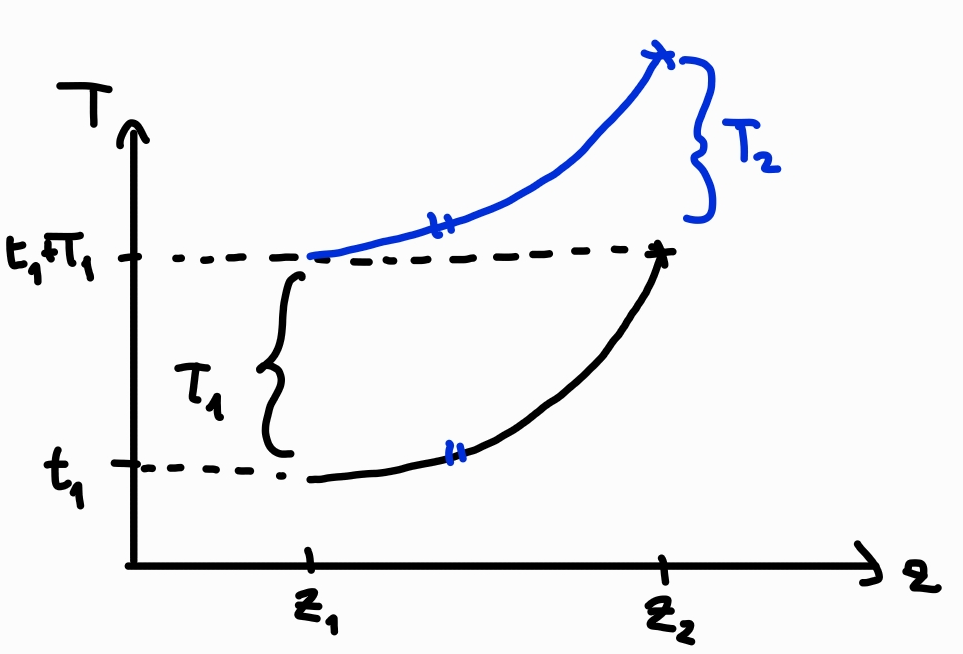
\includegraphics[scale=0.3]{Chapitres/1. Introduction/Images/confusion pure temp.png}
\end{center}
